%******************************************************************************%
%                                                                              %
%                                 Interlude                                    %
%                         for Machine Learning module                          %
%                                                                              %
%******************************************************************************%

% =============================== %
\section*{Interlude}
% =============================== %
\subsection*{Fighting Overfitting... With Regularization}
% ------------------------------- %

\begin{figure}[!h]
    \centering
    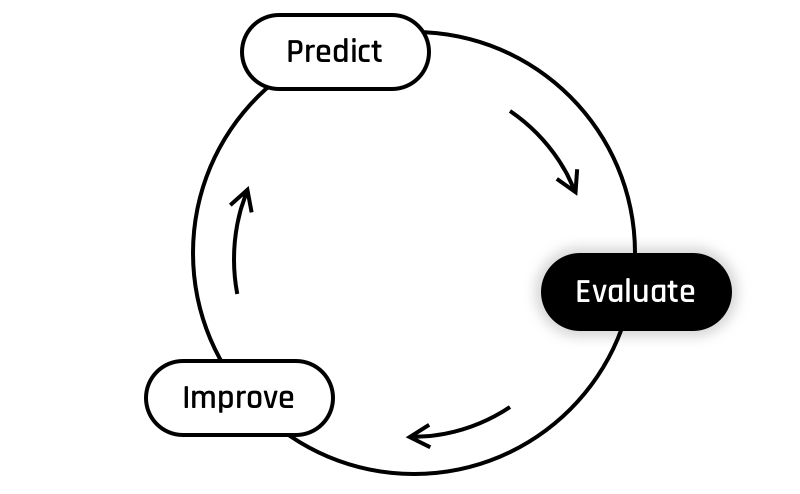
\includegraphics[scale=0.25]{assets/Evaluate.png}
    %\caption{The Learning Cycle - Evaluate}
\end{figure}
\noindent{In the \textbf{module07}, we talked about the problem of \textbf{overfitting} and the necessity 
of splitting the dataset into a \textbf{training set} and a \textbf{test set} in order to spot it.}\\
\\
\textbf{However, being able to detect overfitting does not mean being able to avoid it.}\\
\\
To address this important issue, it is time to introduce a new technique: \textbf{regularization}.
If you remember well, overfitting happens because the model takes advantage of irrelevant 
signals in the training data.\\
\\
The basic idea behind regularization is to \textbf{penalize the model for putting too 
much weight on certain} (usually heavy polynomials) \textbf{features}.\\
\\
We do this by adding an extra term to the loss function formula:

$$
\text{regularized loss function} = \text{loss function} + \frac{\lambda}{2m} \sum_{j = 1}^n \theta_j^2
$$
By doing so, \textbf{we are encouraging the model to keep its} $\theta$ 
\textbf{values as small as possible}.\\
Indeed, the values of $\theta$ \textit{themselves} are now taken 
into account when calculating the loss.\\
\\
$\lambda$ (called \textit{lambda}) is the parameter through which you can modulate how 
reglarization should impact the model's construction.
\begin{itemize}
    \item If $\lambda = 0$, there is no regularization (as we did until now).
    \item If $\lambda$ is very large, it will drive all the $\theta$ parameters to $0$.
\end{itemize}

\info{In the regularization term, the sum starts at $j=1$ because we do NOT 
want to penalize the value of $\theta_0$ (the y-intercept, which doesn't depend on a feature).}

% =============================== %
\subsection*{Be careful!}
% ------------------------------- %
Machine Learning was essentially developped by computer scientists (not mathematicians).\\
\\
This can cause problems when we try to represent things mathematically.
For example: using the $\theta_0$ notation to represent the y-intercept makes things easy 
when we apply the linear algebra trick, \textbf{but} it completely messes up with the overall
 matrix notation!\\
\\
According to that notation, the $X'$ matrix has the following properties: 
\begin{itemize}
    \item its rows, $x'^{(i)}$, follow the mathematical indexing: starting at $1$.
    \item its columns, $x^{'}_j$, follow the computer science indexing: starting at $0$.
\end{itemize}

$$
X' =
\underbrace{
\begin{bmatrix}
1 & x_1^{(1)} & \dots & x_n^{(1)} \\
\vdots & \vdots & \ddots & \vdots \\ 
1 & x_1^{(m)} & \dots & x_n^{(m)} \\ 
\end{bmatrix}  
}_{\begin{matrix}
    j = 0, \dots, n
\end{matrix}}
=     
\left.
\begin{bmatrix}
x_0^{(1)} & x_1^{(1)} & \dots & x_n^{(1)} \\
\vdots & \vdots & \ddots & \vdots \\ 
x_0^{(m)} & x_1^{(m)} & \dots & x_n^{(m)} \\ 
\end{bmatrix}
\right\} i = 1, \dots, m
$$
\\
It's precisely for this reason you keep seeing that $X'$ is of dimension $(m \times (n+1))$.

% =============================== %
\subsection*{Terminology}
% ------------------------------- %
The regularization technique we are introducing here is named \texttt{\textbf{L$_2$ regularization}}, 
because it adds the squared \texttt{\textbf{L$_2$ norm}} of the $\theta$ vector to the loss function.\\
\\
The L$_2$ norm of a given vector $x$, written\\
$$
L_2(x) = ||x||_2 = \sqrt{\sum_i x_i^2} \\
L_2(x)^2 = ||x||_2^2 = \sum_i x_i^2
$$
is its \textbf{euclidean norm} (i.e. the sum of its components squared).\\  

\newpage
There is an infinite variety of norms that could be used as regularization terms, depending on
 the desired regularization effect.\\
Here, we will only use $L_2$, the most common one.

\info{
  The notation $\sum_i$ means: "the sum for all i"\newline
  There is no need to explicitly specify the start and the end of the summation index 
  if we want to sum over all the values of $i$.
  However, it is better to do it anyway as it forces us to make sure of what we are doing.
  And in our case, we do not want to sum over $\theta_0$ ...
}

% =========================================== %
\subsection*{Our old friend vectorization ...}
% ------------------------------------------- %
It is no surprise, we can use vectorization to calculate $\sum_{j = 1}^n \theta_j^2$ more efficiently.\\
\\
It could be a good exercise for you to try to figure it out by yourself.\\
\\
We suggest you give it a try and then check the answer on the next page.\\

\newpage
% =========================================== %
\subsection*{Answers to the Vectorization Problem}
% ------------------------------------------- %
So, how do you vectorize the following?

$$
\sum_{i = j}^n \theta_j^2
$$ 
\\
It's very similar to a \textbf{dot product} of $\theta$ with itself.
The only problem here is to find a way to not take $\theta_0$ into account.\\
\\
Let's construct a vector $\theta'$ with the following rules:\\
\\
$$
\begin{matrix}
\theta'_0 & = 0 &\\
\theta'_j & =  \theta_j & \text{ for } j = 1, \dots, n\\    
\end{matrix}
$$
\\
In other words: 
$$
\\
\theta' = \begin{bmatrix}
  0 \\
  \theta_1 \\
  \vdots \\
  \theta_n
\end{bmatrix}
$$
\\
This way, we can perform the dot product without having $\theta_0$ interfering in our calculations:

$$
\begin{matrix}
\theta' \cdot \theta' & = & 
\begin{bmatrix}
  0 \\
  \theta_1 \\
  \vdots \\
  \theta_n
\end{bmatrix} \cdot \begin{bmatrix}
  0 \\
  \theta_1 \\
  \vdots \\
  \theta_n
\end{bmatrix} \\ 
\\
& = & 0 \cdot 0 + \theta_1 \cdot \theta_1 + \dots + \theta_n \cdot \theta_n \\ 
\\
& = & \sum_{j= 1}^n \theta_j^2
\end{matrix}
$$
